\documentclass[times, utf8, seminar]{fit}

%\batchmode
%\usepackage{booktabs}
\usepackage{listings}
\usepackage{longtable}
\usepackage{xcolor}
\usepackage{float}
\usepackage{enumitem}
\usepackage{hyperref}
\usepackage{enumerate}
\usepackage{graphicx}
\usepackage{etoolbox}
\usepackage{datetime}
\usepackage{needspace}
\usepackage{titlesec}
%\usepackage{hyperref}
%\titleformat{\chapter}[display]{\normalfont\huge\bfseries}{\chaptertitlename\ \thechapter}{20pt}{\Huge}

\begin{document}
\widowpenalty=300
\clubpenalty=300

\lstset{
  language=bash,
  backgroundcolor=\color{gray!25},
  basicstyle=\ttfamily \footnotesize,
  breaklines=true,
  prebreak=\raisebox{0ex}[0ex][0ex] \hookleftarrow,
  columns=fullflexible
}


% this alters "before" spacing (the second length argument) to 0
%\titlespacing*{\chapter}{0pt}{0pt}{40pt}

% this changes "before" spacing back to its default of 50pt
%\titlespacing*{\chapter}{0pt}{50pt}{40pt}}

%\titlespacing*{\chapter}{0pt}{-50pt}{18pt}
%\titleformat{\chapter}[display]{\normalfont\huge\bfseries}{\chaptertitlename\ \thechapter}{20pt}{\Huge}

\title{Agilni \emph{software development},\newline GIT SCM}

\author{Ernad Husremović}
\brindex{DL 2792}
\verzija {0.0.1}

\mentor{mr. Adil Joldić}

\maketitle

\tableofcontents

%\listoftables
%\listoffigures
\newpage

\begin{abstract}

Dokument na bazi konkretnog primjera\footnote{"HOWTO" stil} objašnjava uobičajeni developerski `workflow' pri korištenju GIT `Source Code Management' (SCM) alata. 
U primjeru se koriste GIT web servisi `Github'\footnote{\url{https://www.github.com}} i `Gitlab'\footnote{\url{https://gitlab.knowhow.out.ba}, \url{http://gitlabhq.com}}.
Čitalac će upoznati osnovne operacije GIT klijenta i način korištenje navedenih web servisa.


\keywords{open source software, OSS, Source code management, SCM, DSCM, Version control, GIT}
\end{abstract}

% abstract end

\chapter{Uvod}
\vspace*{-0.7cm}

\section{`Source code management' (SCM) software}

`Source code management' (SCM) software obezbjeđuje pohranu različitih verzija programskog koda u zajednički repozitorij. 
Iako je prvobitna ovih alata bilo čuvanje programskog koda, oni se mogu koriste za za pohranu (verzioniranje) svih artifakta softverskog projekta uključujući dokumentaciju, dijagrame, binarni kod.
Ovaj software se često naziva i `Version control' software.

Sa stanovišta arhitekture, SCM sistemi se dijele na centralizovane i distribuirane (DSCM).

\subsection{Centralizirani (mrežni) SCM}

Najpoznatiji predstavnici su `CVS' i `Subversion'. `CVS' je među prvim SCM alatima-ima koji je postigao veliku popularnost.

`Subversion' je uveo značajna tehnička unapređenja, ali je arhitekturalno identičan svom predhodniku. Oba alata su `open source' software (OSS).

Njihova glavna karakakteristika je klasična `client-server' arhitektura. Da bi se SCM operacije na klijentu izvršavale, neophodna je dostupnost SCM servera.
Razlog je taj što se istorija promejan nalazi isključivo na serveru.

Ova karakteristika danas se smatra ključnim nedostatkom centraliziranih SCM-ova

\subsection{Distribuirani SCM (DSCM)}

Distribuirani SCM-omi imaju potpuno različitu arhitekturu. Baza promjena nalazi se na svakom klijentu.
Sami developeri određuju funkciju pojedinačnih repozitorija. Glavni repozitorij (`upstream') je dostupan udaljenim klijentima.
Razmjena podataka (`commit'-a) se vrši sistemom sinhronizacije repozitorija klijenta i servera (`merge' proces). 
Usljed nedostatka centralnog repozitorija, sasvim su normalne situacije u kojima se repozitoriji koji se usaglašavaju - sinhronizuju u stanju konflikta.
U tom slučaju potrebno je izvršiti manuelni ''merge'' proces kojim se promjene primljene iz različitih izvora usaglašavaju.
Iako ovaj koncept na prvi pogled djeluje kao izvor velikih glavobolja, pravilna primjena DSCM alatima daje veliku fleksibilnost i niz prednosti u odnosu na centralizirane SCM-ove.

Jedna od ključnih prednosti DSM-ova je `off-line' režim rada, kao posljedica činjenice da svaki korisnik ima sopstveni lokalni repozitorij promjena.

\chapter{Gitlab servis i git klijent}
\vspace*{-0.7cm}

\section{Gitlab servis}

"Gitlab"\footnote{\url{http://gitlabhq.com}} je OSS projekat, po mnogo čemu "klon" popularnog "Github" servisa. 
Autor nudi komercijalni servis \href{https://gitlab.com}{\color{blue}{''gitlab.com''}} baziran na ovom serveru.

S obzirom da se radi OSS software-u, korisnici bez ograničenja mogu kreirati sopstvene "gitlab" server-e.
U ovom materijalu se koristi server \href{https://gitlab.knowhow.out.ba}{\color{blue}{''gitlab.knowhow.out.ba''}} instaliran upravo na taj način.

\section{git klijent}

Tvorac git-a je kreator Linux-a, Linus Torvalds.
Prve verzije git-a su se mogle koristiti samo ''unix-like'' sistemima\footnote{git se mogao koristiti na Windows-ima putem ''cygwin'' emulacijskog sloja, ali je rad sa iole većim repozitorijem bio veoma spor}. 
Popularnost i otvorenost projekta je brzo rezultirala i ''native'' git verzijom klijenta.

U našem primjeru je radi jednostavnosti korištenja na ''Windows'' klijentu korišten \href{http://railsinstaller.org/}{\color{blue}{''Rails installer''}}. 
''Rails installer'' sadrži kompletno ruby/rails/git razvojno okruženje za ''Windows'' XP/W7 OS.

Nakon instalacije ''Rails installer'' traži podatke o korisniku, te kreira ssh ključ koji će se koristiti za povezivanje sa git serverom putem ssh protokola:

\begin{lstlisting}
# Rails Environment Configuration.

Your git configuration is incomplete.
user.name and user.email are required for properly using git and services such
as GitHub ( http://github.com/ ).

 Please enter your name, for example mine is: Wayne E. Seguin
name > Bakir Husremovic                   <<<<<<<<<<<<<<<< unijeti <<<<<<<<<<<<<<<<
Setting user.name to Bakir Husremovic

 Please enter your email address, for example mine is: wayneeseguin@gmail.com
email > bakir.husremovic@gmail.com        <<<<<<<<<<<<<<<< unijeti <<<<<<<<<<<<<<<<
Setting user.email to bakir.husremovic@gmail.com
---
git:
  user.name:  Bakir Husremovic
  user.email: bakir.husremovic@gmail.com
  version:    git version 1.7.9.msysgit.0

ruby:
  bin:        C:/RailsInstaller/Ruby1.9.2/bin/ruby.exe
  version:    ruby 1.9.3p125 (2012-02-16) [i386-mingw32]

rails:
  bin:        C:/RailsInstaller/Ruby1.9.2/bin/rails.bat
  version:    Rails 3.2.1

ssh:
  public_key_location: C:\Documents and Settings\hbakir/.ssh/id_rsa.pub  <<<<<<<<<<<
  public_key_contents: ssh-rsa AAAAB3NzaC1yc2EAAAABIwAAAQEAwSrpSeOyx7OaWZ7b6ZZ8
  ....
  45tg6Y18rxVgzOgK6YxsZP+qOuOtCGK4J23GPb/3fIRRqOYVx5UpftMqq0p0e54GUQOcr0bS+/ooYNC
Q== Bakir Husremovic <bakir.husremovic@gmail.com>
\end{lstlisting}

\subsection{Gitlab ssh pristup}

Gitlab web servis obezbjeđuje smještaj git repozitorija na server putem ssh i http(s) protokola. 
Takođe obezbjeđuje upravljanje korisnicima, pregled git repozitorija kao i niz drugih funkcija vezanih za rad na softverskim projektima\foonote{''Issues'', ''Wikies'', ''Code Snippets'', 'Code comments'}.
U ovom materijalu ćemo se fokusirati na git funkcije. 

Korisnik na svom računu podešava ssh ključ:

\begin{figure}[H]
\centering
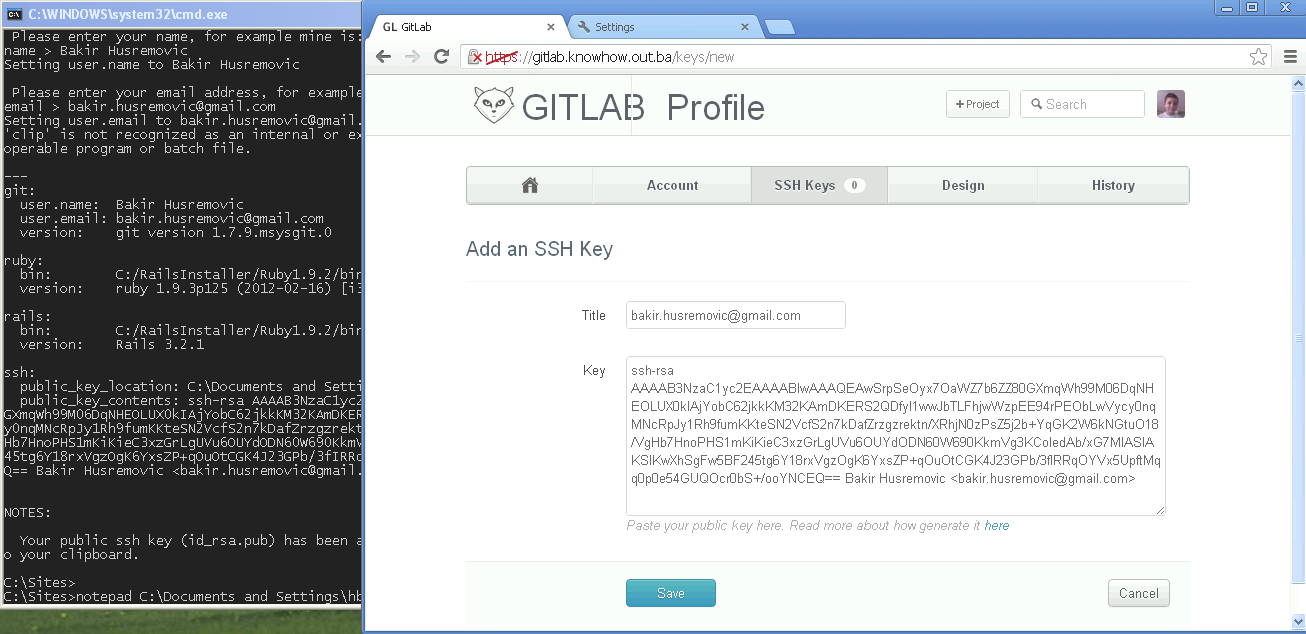
\includegraphics[width=15cm]{img/gitlab_ssh_profile.png}
\caption{Gitlab ssh profil}
\end{figure}

\section{Git workflow}

\subsection{Novi projekat}

Kreirajmo naš ''helo\_ruby'' projekat.

\begin{figure}[H]
\centering
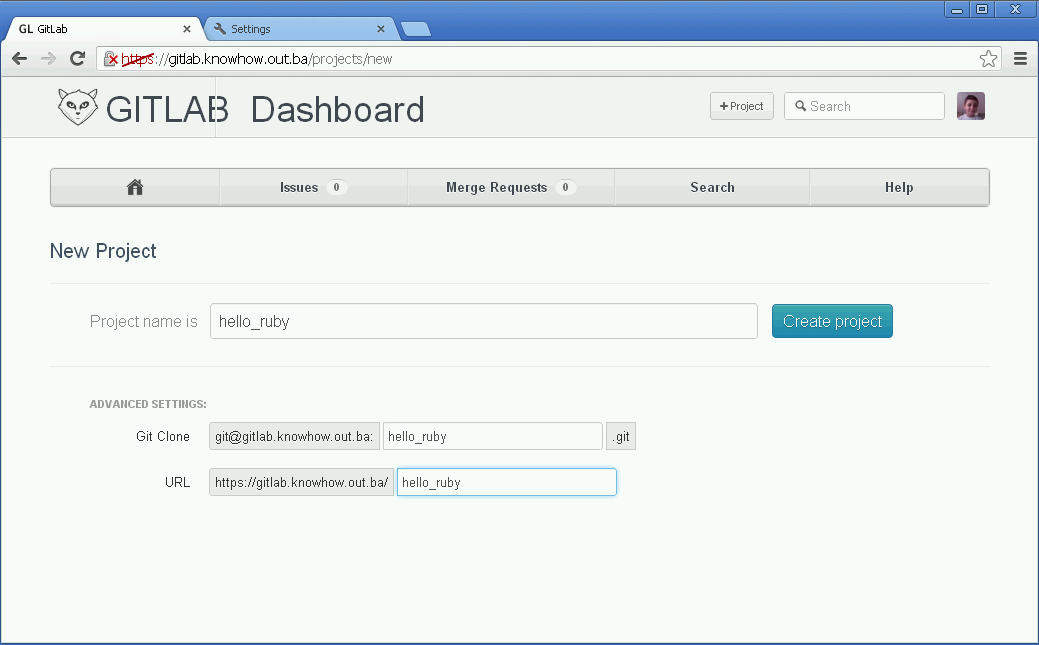
\includegraphics[width=15cm]{img/gitlab_new_project.png}
\caption{Gitlab: novi projekat}
\end{figure}


\begin{figure}[H]
\centering
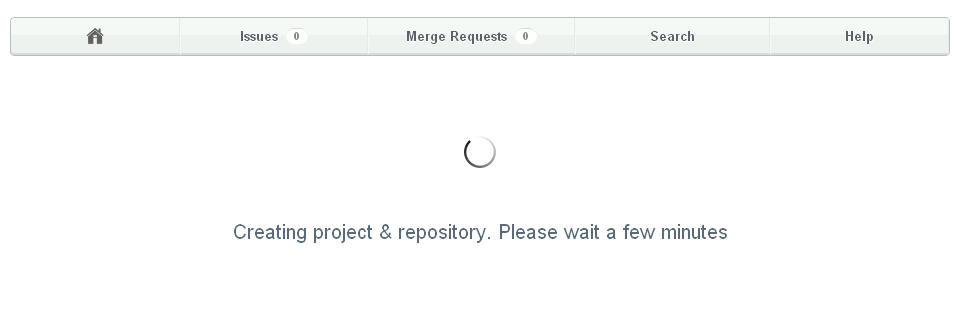
\includegraphics[width=15cm]{img/gitlab_new_project_2.png}
\caption{Gitlab: novi projekat - kreiranje git repozitorija}
\end{figure}

Nakon što je git repozitorij kreiran, dobijamo informacije o operacijam koje se obavljaju na remote klijentu za kreiranje i pristup git repozitoriju:

\begin{figure}[H]
\centering
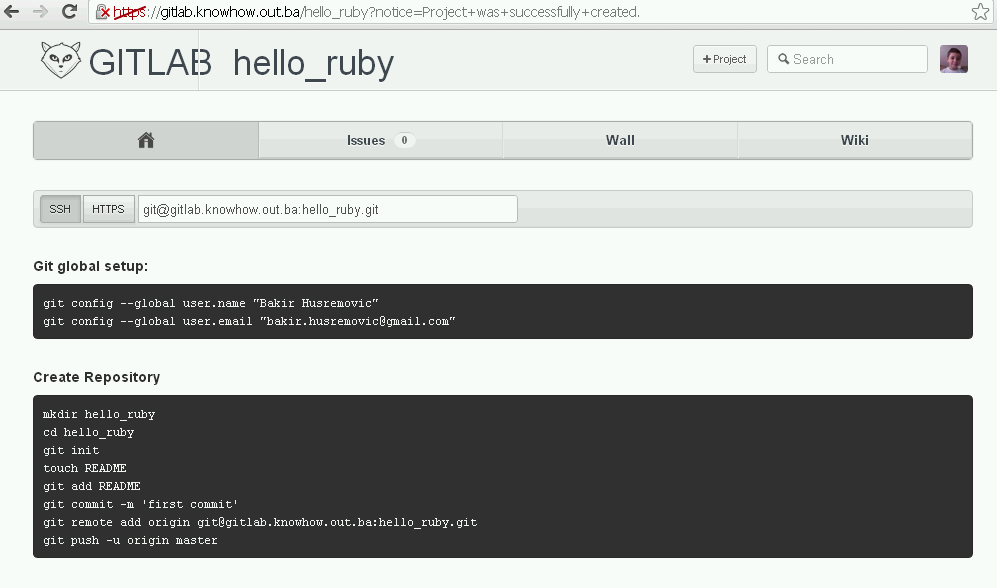
\includegraphics[width=15cm]{img/gitlab_new_project_3.png}
\caption{Gitlab: informacije o pristupu git prepozitiriju}
\end{figure}

\section{Development}

\subsection{Prvi ''commit''}

\begin{figure}[H]
\centering
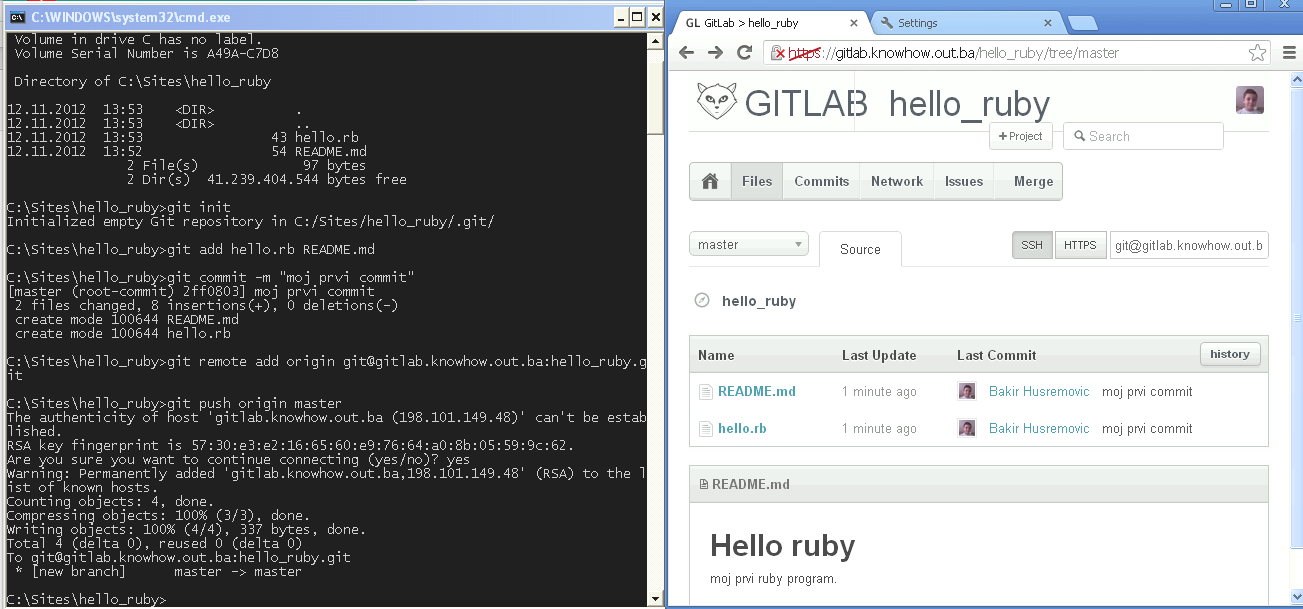
\includegraphics[width=15cm]{img/gitlab_first_commit.png}
\caption{Prve operacije na git repozitoriju: add, commit, push}
\end{figure}


Na konzoli smo napravili prve testove našeg hello.rb programa. Takođe, na gitlab konzoli, nakon "push" operacije programski kod vidimo i na serveru:

\begin{figure}[H]
\centering
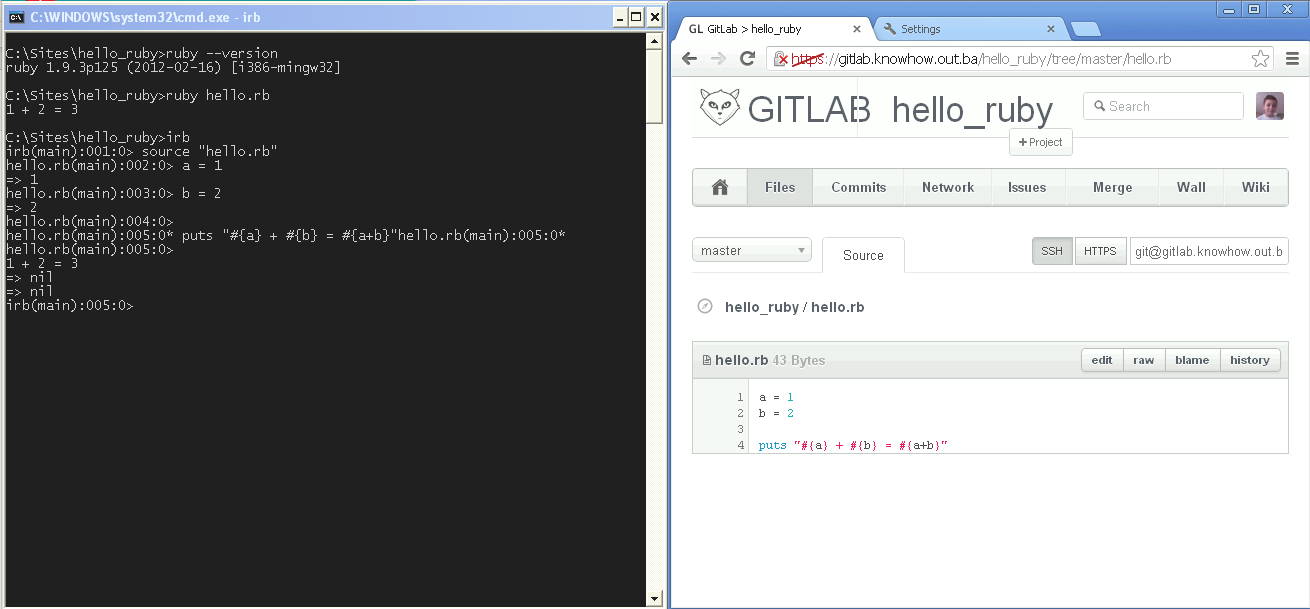
\includegraphics[width=15cm]{img/gitlab_first_commit_2.png}
\caption{Izvorni kod našeg programa je na gitlab serveru}
\end{figure}

\begin{figure}[H]
\centering
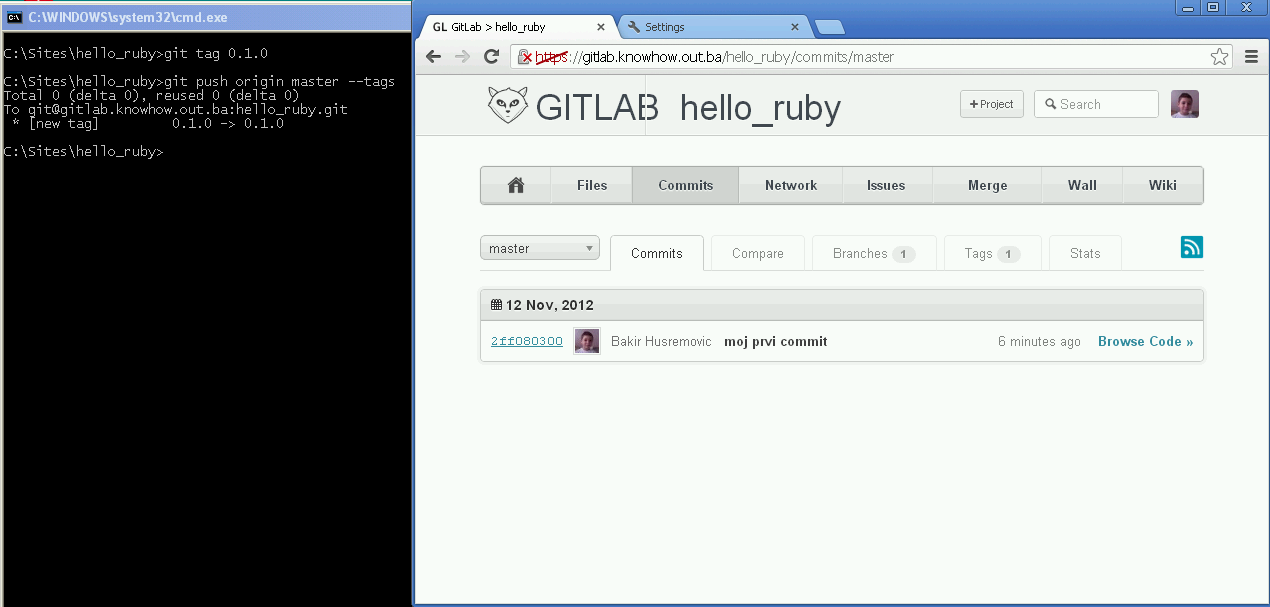
\includegraphics[width=15cm]{img/gitlab_tag_first_release.png}
\caption{''Označavamo'' prvu verziju našeg software-a: release 0.1.0}
\end{figure}

Napravimo pregled izvršenih operacija:
\begin{enumerate}
  \item \texttt{git init} - kreiramo .git direktorij, lokalni git repozitorij
  \item \texttt{git remote add origin} - navodimo lokaciju našeg udaljenog - serverskog git repozitorija 
  \item \texttt{git add <ime fajla>} - dodajemo fajlove u lokalni repozitorij
  \item \texttt{git commit} - sve što unutar projekta dodali/promijenili smještamo u lokalni repozitorij
  \item \texttt{git tag} - ''tagiramo'' (označavamo) verziju 0.1.0
  \item \texttt{git push origin master} - šaljemo master\footnote{novokreirani git repozitorij uvijek ima ''master'' branch - to je podrazumjevani (eng. default) branch} ''branch'' na server 
\end{enumerate}

Nakon svih ovih operacija možemo vidjeti pregled operacija koje su do sada izvršene na projektu:

\begin{figure}[H]
\centering
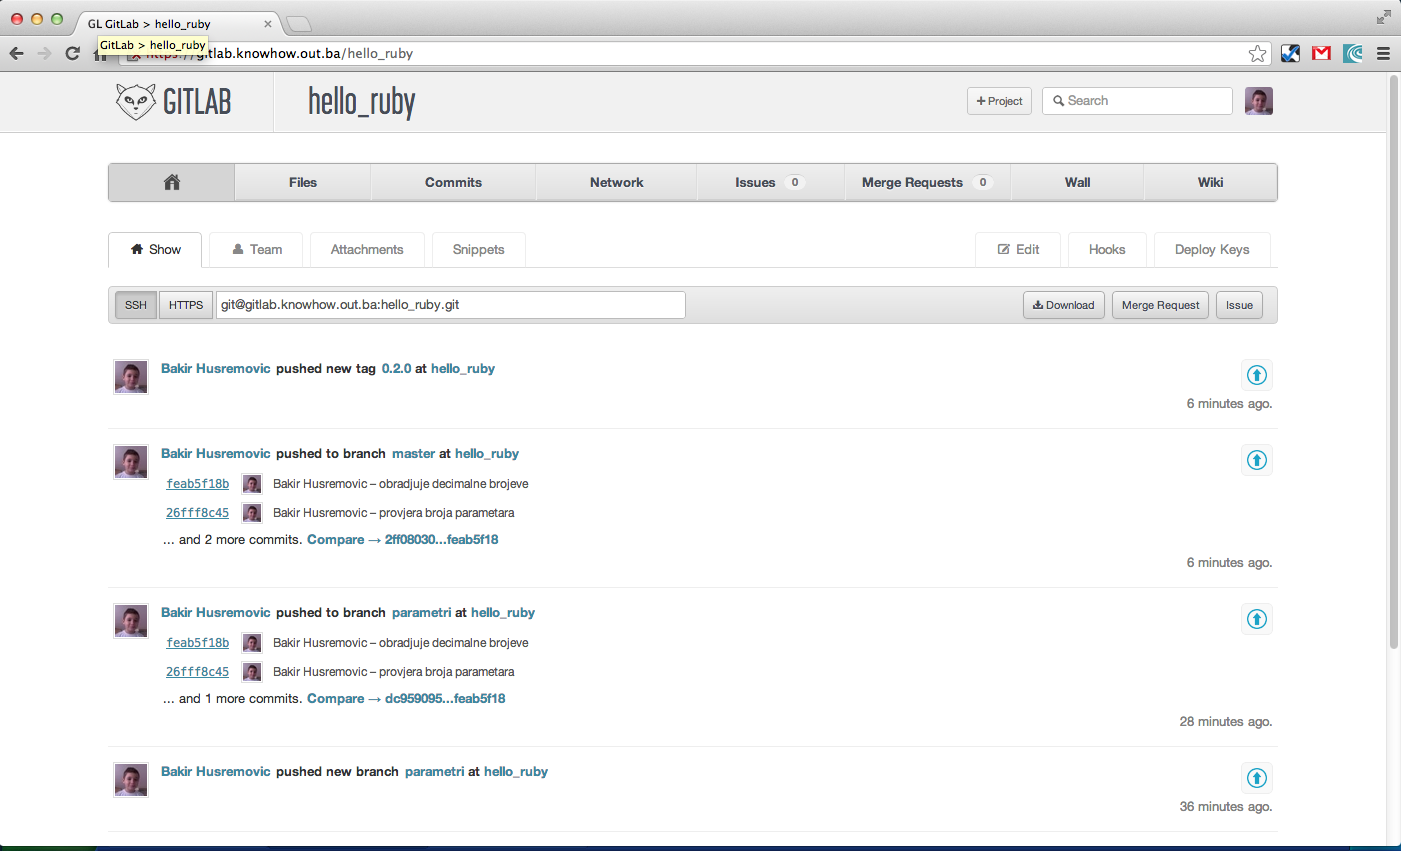
\includegraphics[width=15cm]{img/gitlab_project_show.png}
\caption{Glavne aktivnosti na projektu}
\end{figure}


\begin{figure}[H]
\centering
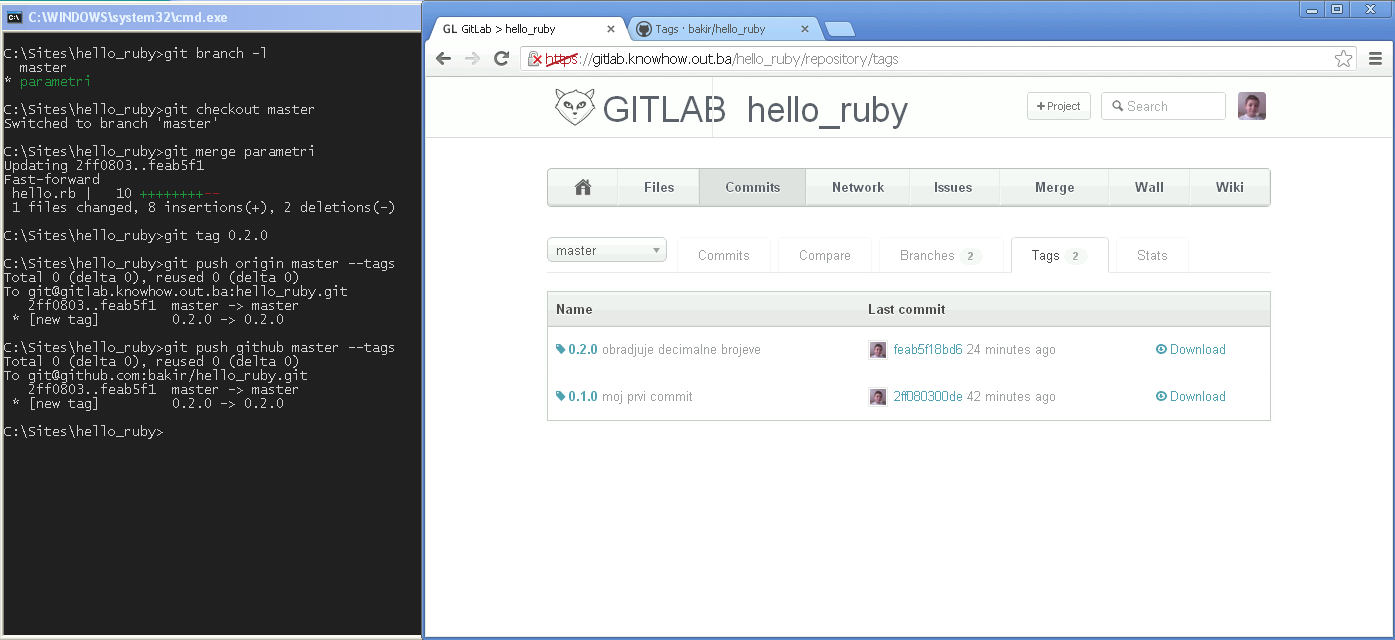
\includegraphics[width=15cm]{img/gitlab_tags.png}
\caption{Pregled tagova}
\end{figure}


\section{Github public mirror}

Glavni repozitorj projekta nalazi se na gitlab serveru. Međutim, "gitlab" ne omogućava anonimni pristup repozitorijima.

Ništa nas ne sprječava da na drugom git serveru kreiramo mirror našeg repozitorija.

To ćemo i učiniti. Otvorićemo account na github-u i na njemu kreirati hello\_ruby projekat.

\subsection{Githu account}

Kreiranje novog korisničkog računa na github-u:

\begin{figure}[H]
\centering
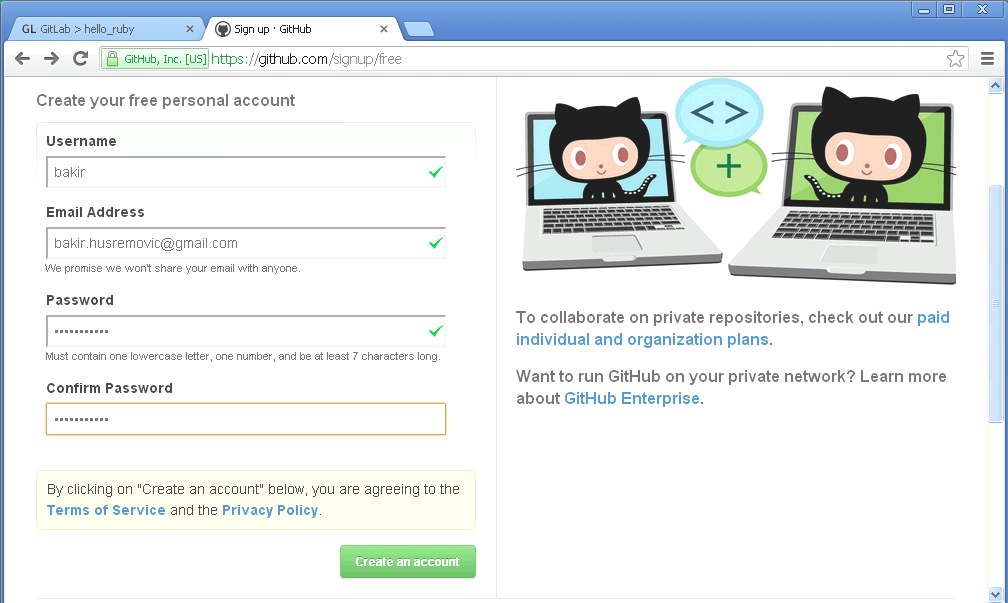
\includegraphics[width=15cm]{img/github_prijava.png}
\caption{Github prijava}
\end{figure}

\subsection{Github ssh postavke}

\begin{figure}[H]
\centering
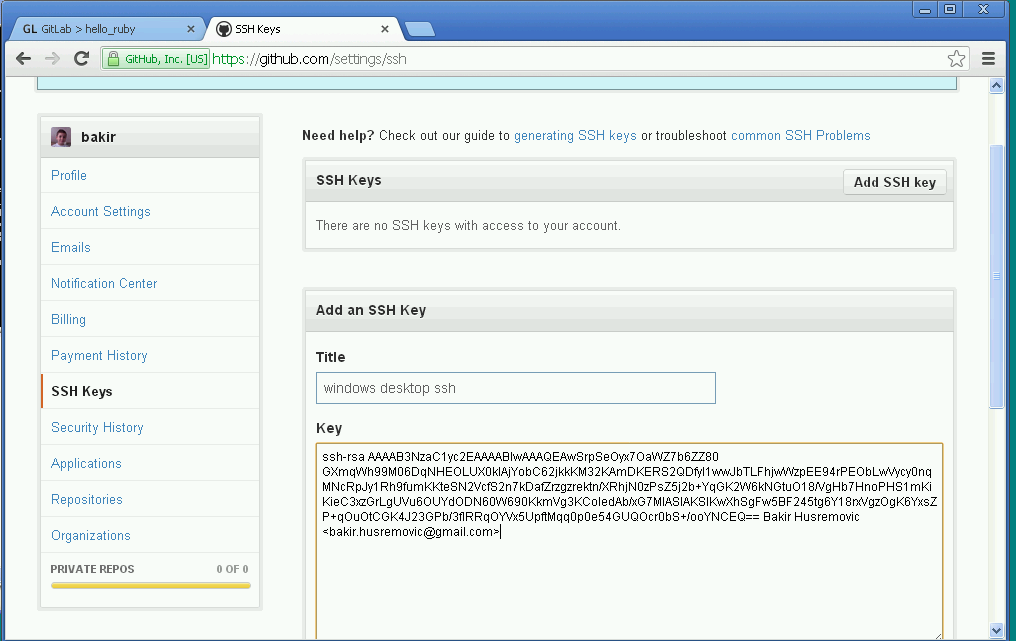
\includegraphics[width=15cm]{img/github_ssh_profile.png}
\caption{Github ssh profil}
\end{figure}

\begin{figure}[H]
\centering
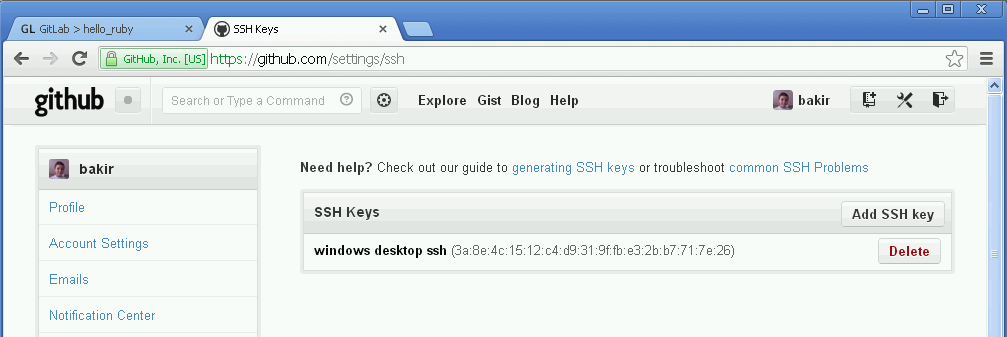
\includegraphics[width=15cm]{img/github_ssh_profile_2.png}
\caption{Github ssh profil /2}
\end{figure}

\subsection{Github kreiranje repozitorija}

\begin{figure}[H]
\centering
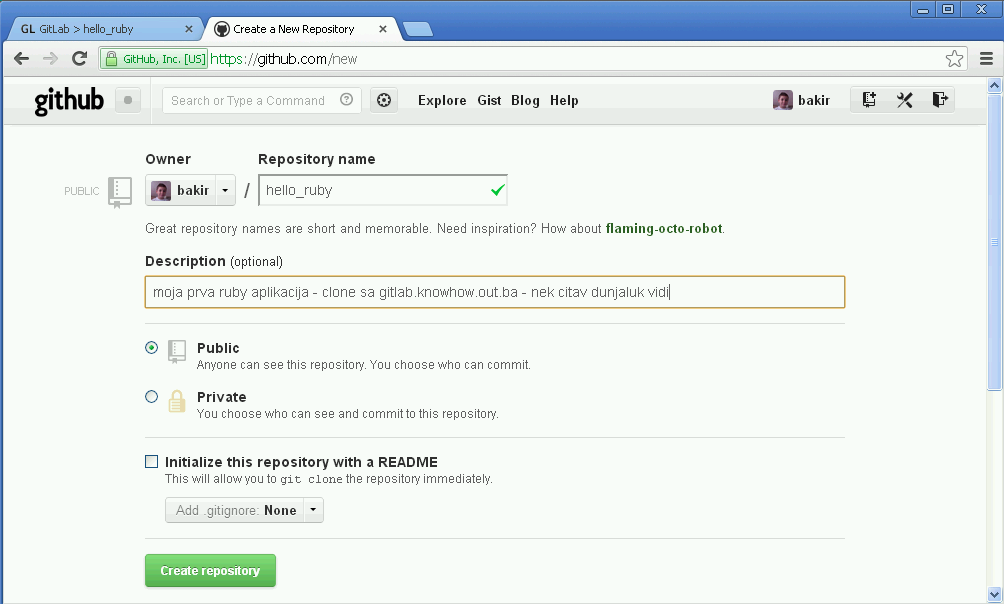
\includegraphics[width=15cm]{img/github_new_repos.png}
\caption{Github novi repozitorij}
\end{figure}

\begin{figure}[H]
\centering
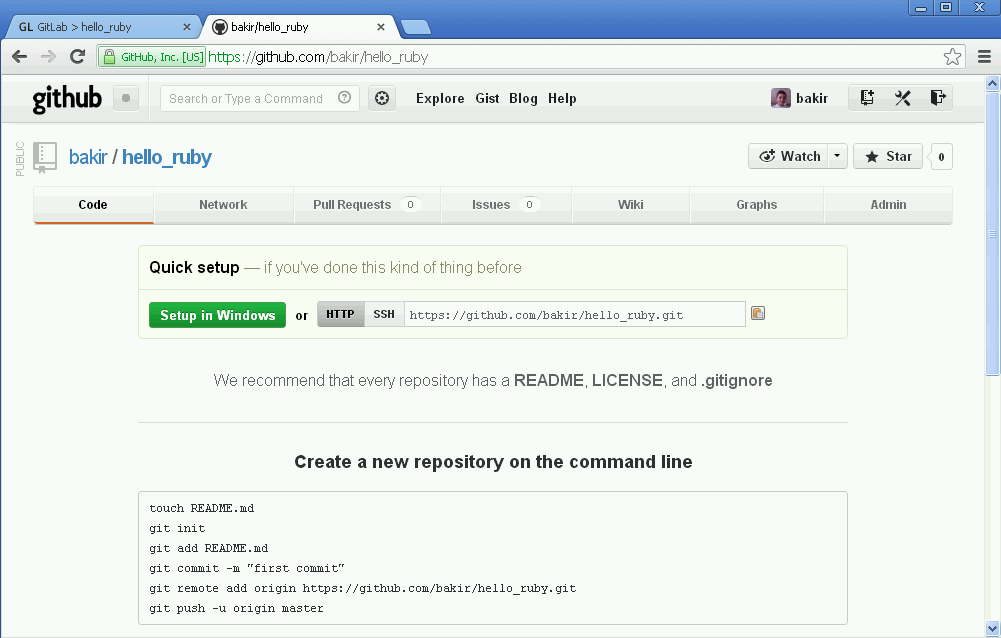
\includegraphics[width=15cm]{img/github_new_repos_2.png}
\caption{Github novi repozitorij / 2}
\end{figure}

\subsection{Kreiranje mirrora projekta na github-u}

\begin{figure}[H]
\centering
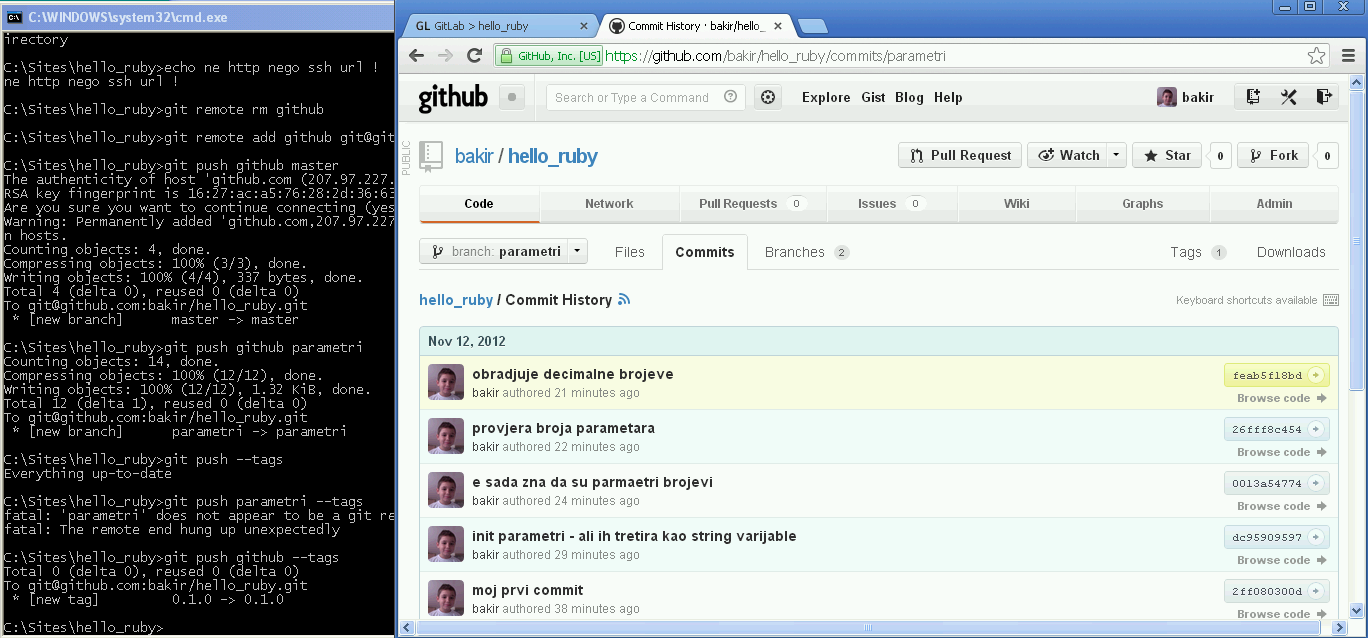
\includegraphics[width=15cm]{img/github_push_branches_and_tags.png}
\caption{Pošalji sve branchove i tag-ove na github repozitorij}
\end{figure}

\section{Nova verzija}

Vrijeme je za novu verziju, zato vršimo tagiranje git repozitorija sa ''0.2.0'':

\begin{figure}[H]
\centering
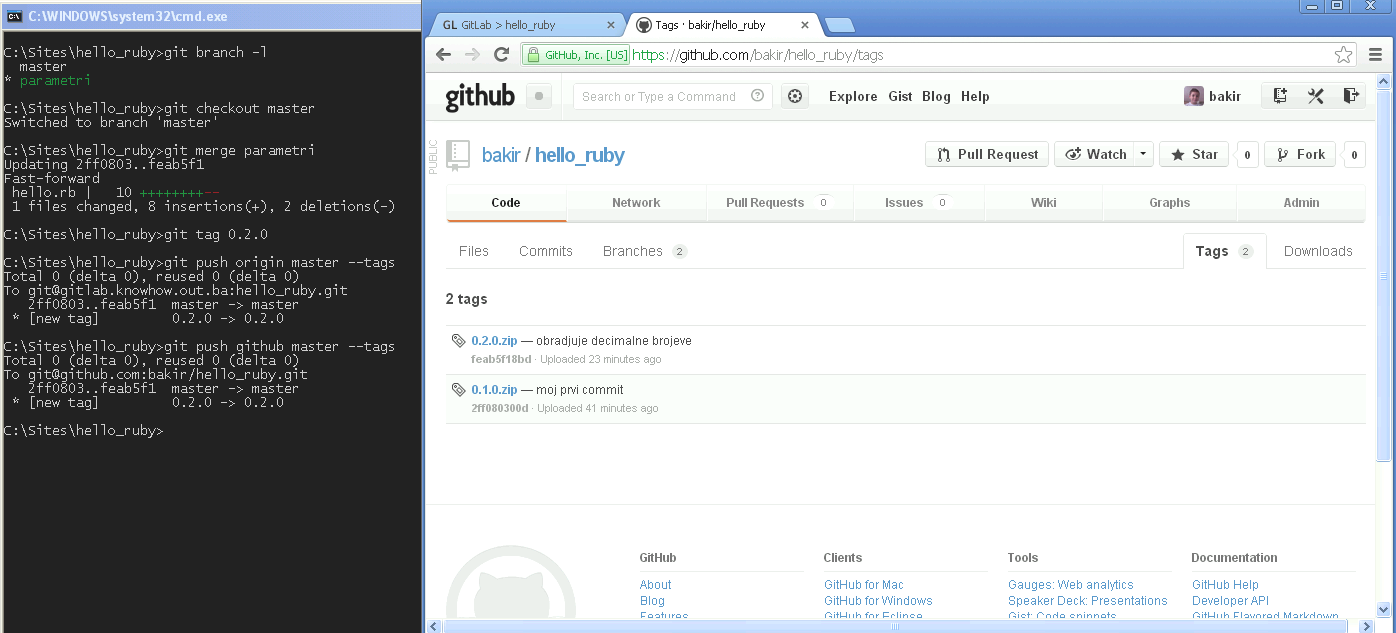
\includegraphics[width=16cm]{img/github_new_tag.png}
\caption{Github - novi tag}
\end{figure}


\section{Compare}

\begin{figure}[H]
\centering
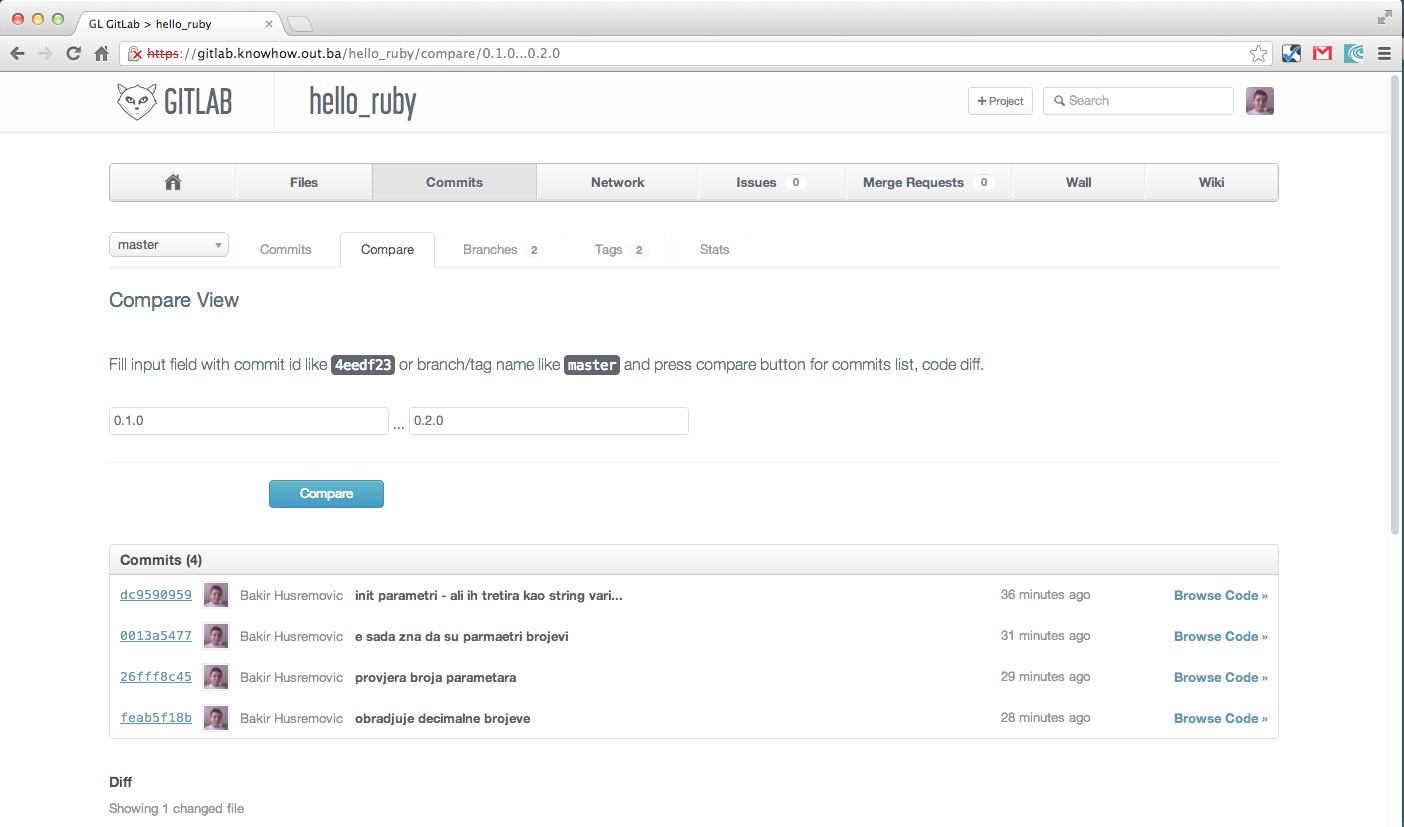
\includegraphics[width=15cm]{img/gitlab_compare.png}
\caption{Gitlab uporedi dvije verzije}
\end{figure}


\begin{figure}[H]
\centering
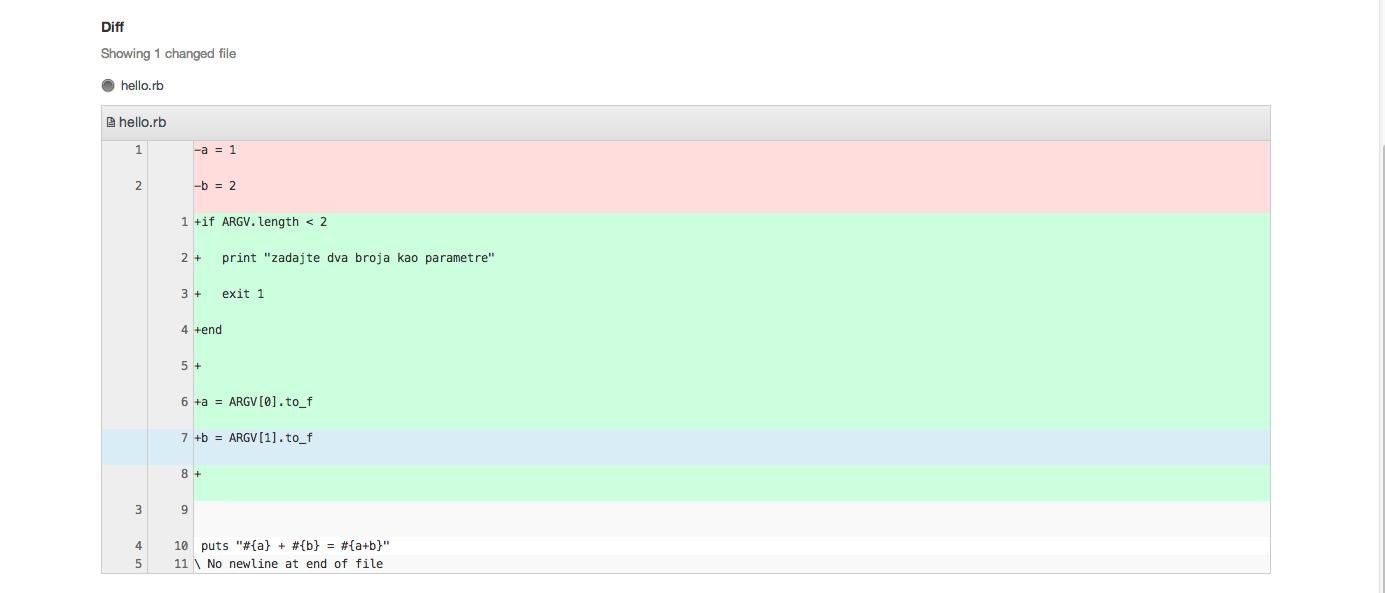
\includegraphics[width=15cm]{img/gitlab_compare_2.png}
\caption{Gitlab uporedi dvije verzije /2}
\end{figure}


\begin{figure}[H]
\centering
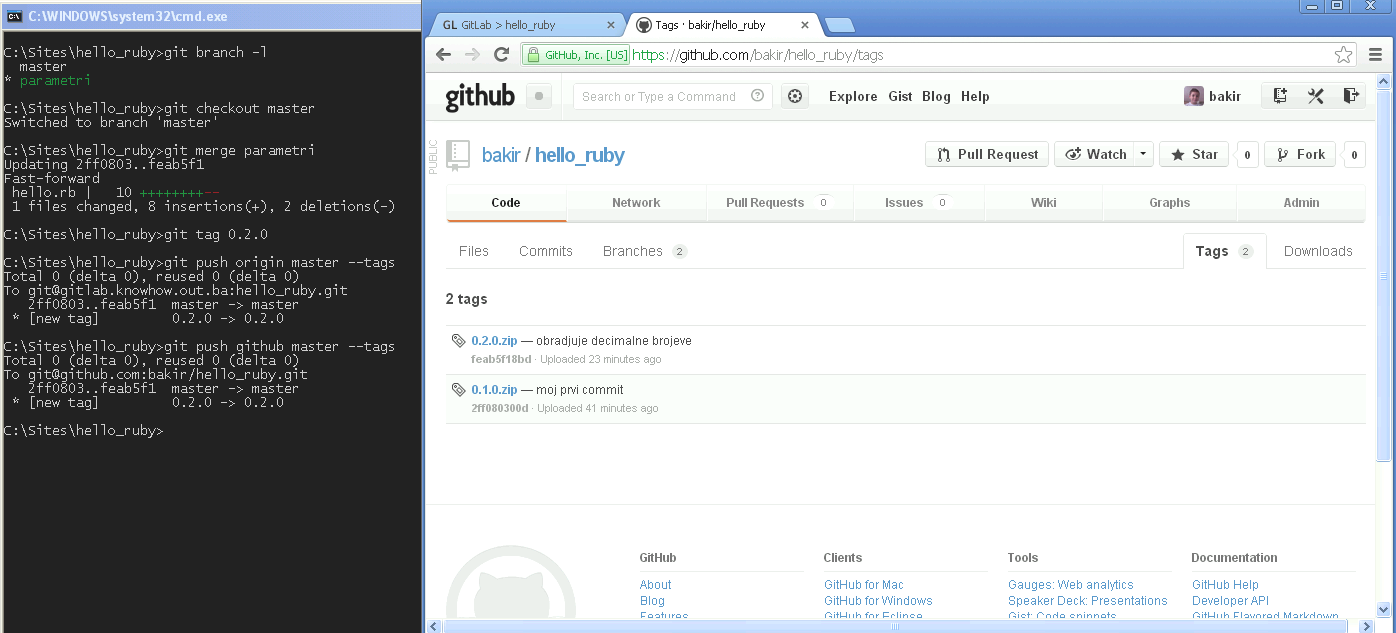
\includegraphics[width=16cm]{img/github_new_tag.png}
\caption{Github - novi tag}
\end{figure}


\section{Novi developer}

\subsection{Gitlab: Uključenje novog developera u projekat}

Vlasnik projekta ''hello\_ruby'' Bakir uključuje novog developera u projekat Ernad:

\begin{figure}[H]
\centering
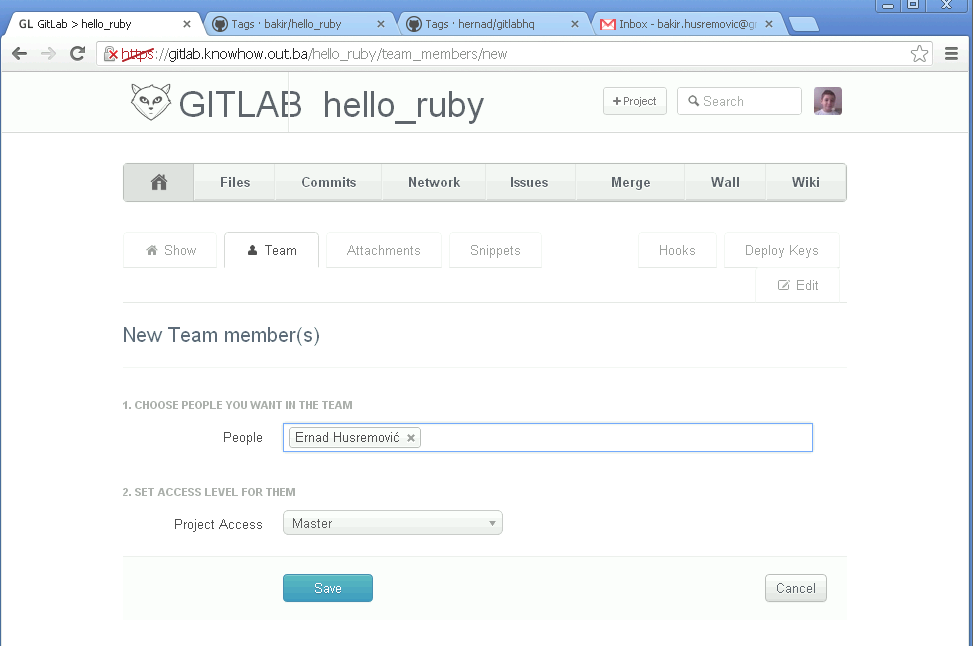
\includegraphics[width=15cm]{img/gitlab_add_new_member_to_project.png}
\caption{Gitlab: dodaj novog člana u projekat}
\end{figure}

\begin{figure}[H]
\centering
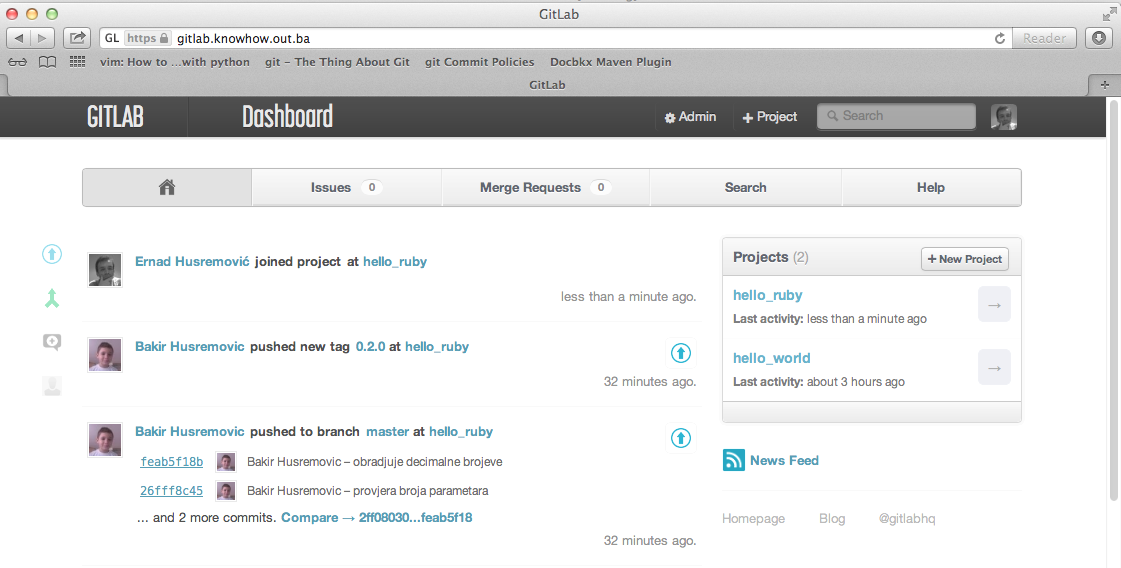
\includegraphics[width=15cm]{img/gitlab_add_new_member_to_project_2.png}
\caption{Gitlab dodaj novog člana u projekat 2}
\end{figure}

\section{email notifikacija}

Developeri primaju email notifikacije o svim bitnim događajima na projektu:

\begin{figure}[H]
\centering
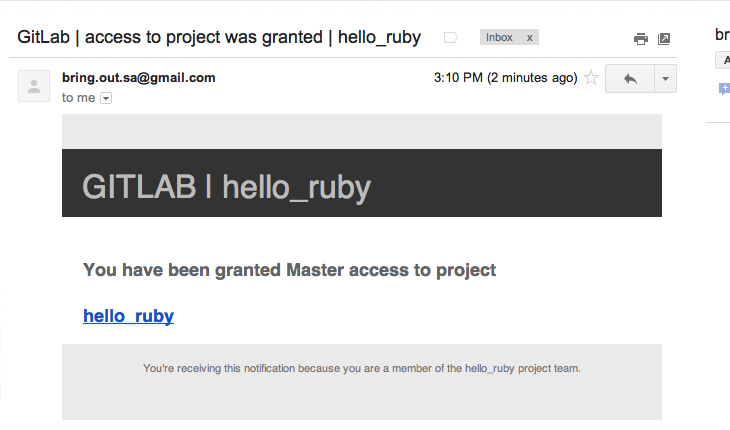
\includegraphics[width=15cm]{img/gitlab_email_notification.png}
\caption{Gitlab email notifikacija}
\end{figure}


\subsection{git clone}

Prvi korak novog developera je kloniranje repozitorija projekta na svoj desktop. 

Novi developer koristi Ubuntu linux desktop.

\setlength{\parindent}{0cm}

hernad@agile\_dev\_env\$ \texttt{git clone git@gitlab.knowhow.out.ba:hello\_ruby.git}
\begin{lstlisting}
Cloning into 'hello_ruby'...
remote: Counting objects: 16, done.
remote: Compressing objects: 100% (15/15), done.
remote: Total 16 (delta 1), reused 0 (delta 0)
Receiving objects: 100% (16/16), done.
Resolving deltas: 100% (1/1), done.
\end{lstlisting}

hernad@hello\_ruby\$ \texttt{git branch -r}
\begin{lstlisting}
  origin/HEAD -> origin/master
  origin/master
  origin/parametri
\end{lstlisting}


hernad@hello\_ruby\$ \texttt{git branch parametri}
\begin{lstlisting}
  origin/HEAD -> origin/master
  origin/master
  origin/parametri
\end{lstlisting}


hernad@hello\_ruby\$ \texttt{git checkout parametri}
\begin{lstlisting}
Branch parametri set up to track remote branch parametri from origin.
Switched to a new branch 'parametri'
\end{lstlisting}


hernad@hello\_ruby\$ \texttt{git checkout master}
\begin{lstlisting}
Switched to branch 'master'
\end{lstlisting}


hernad@hello\_ruby\$ \texttt{git branch -l}
\begin{lstlisting}
* master
  parametri
\end{lstlisting}

hernad@hello\_ruby\$ \texttt{git tag -l}
\begin{lstlisting}
0.1.0
0.2.0
\end{lstlisting}

Pregled lokalnog ''commit'' log-a:

hernad@hello\_ruby\$ \texttt{git log}
\begin{lstlisting}
commit 585688af924873852d72a0b9ccad16952c95fef0
Author: Ernad Husremovic <hernad@bring.out.ba>
Date:   Mon Nov 12 15:42:26 2012 +0100

    uputstvo

commit 71f0f17df4b4d0dcbca50034d638bc6bfae50424
Author: Ernad Husremovic <hernad@bring.out.ba>
Date:   Mon Nov 12 15:38:46 2012 +0100

    zaokruzenje pravi probleme
    
    ruby hello.rb
    treba zadati dva broja kao parametre aplikacije
    Unesite varijablu a: 1.1
    
    Unesite varijablu b: 2.2
    1.1 + 2.2 = 3.3000000000000003

commit 8e1c0bd154dd6a57d67266aee5f1f005c4aea603
Author: Ernad Husremovic <hernad@bring.out.ba>
Date:   Mon Nov 12 15:35:18 2012 +0100

    ako ne navedes parametre, procitaj ih sa konzole

commit feab5f18bd616ea7b4278024579e0a7aa728f448
Author: Bakir Husremovic <bakir.husremovic@gmail.com>
Date:   Mon Nov 12 14:15:45 2012 +0100

    obradjuje decimalne brojeve
\end{lstlisting}


\subsection{Kreriranje novog ''branch''-a}

Novi developer kreće u izradu varijante aplikacije koja će preuzeti parametre kod poziva aplikacije.

Da ne bi ometao rad na ''master'' branchu-u, otvara branch ''parametri''.

hernad@hello\_ruby\$ \texttt{git branch babo}

hernad@hello\_ruby\$ \texttt{git checkout babo}

Pošaljimo na server novi branch ''babo'':

hernad@hello\_ruby\$ \texttt{git push origin babo}
\begin{lstlisting}
Counting objects: 12, done.
Delta compression using up to 8 threads.
Compressing objects: 100% (9/9), done.
Writing objects: 100% (9/9), 1.42 KiB, done.
Total 9 (delta 1), reused 0 (delta 0)
To git@gitlab.knowhow.out.ba:hello_ruby.git
 * [new branch]      babo -> babo
\end{lstlisting}

\section{Zajednički rad}


C:\\Sites\\hello\_ruby> \texttt{git pull}
\begin{lstlisting}
remote: Counting objects: 12, done.
remote: Compressing objects: 100% (9/9), done.
remote: Total 9 (delta 1), reused 0 (delta 0)
Unpacking objects: 100% (9/9), done.
From gitlab.knowhow.out.ba:hello_ruby
 * [new branch]      babo       -> origin/babo
You asked me to pull without telling me which branch you
want to merge with, and 'branch.master.merge' in
your configuration file does not tell me, either. Please
specify which branch you want to use on the command line and
try again (e.g. 'git pull <repository> <refspec>').
See git-pull(1) for details.

If you often merge with the same branch, you may want to
use something like the following in your configuration file:
    [branch "master"]
    remote = <nickname>
    merge = <remote-ref>

    [remote "<nickname>"]
    url = <url>
    fetch = <refspec>

See git-config(1) for details.
\end{lstlisting}

C:\\Sites\\hello\_ruby> \texttt{git branch -r}
\begin{lstlisting}
  github/master
  github/parametri
  origin/babo
  origin/master
  origin/parametri
\end{lstlisting}

C:\\Sites\\hello\_ruby> \texttt{git checkout babo}
\begin{lstlisting}
Branch babo set up to track remote branch babo from origin.
Switched to a new branch 'babo'
\end{lstlisting}

C:\\Sites\\hello\_ruby> \texttt{git branch -l}
\begin{lstlisting}
* babo
  master
  parametri
\end{lstlisting}

C:\\Sites\\hello\_ruby> \texttt{git checkout master}
\begin{lstlisting}
Switched to branch 'master'

C:\Sites\hello_ruby>git merge babo
Updating feab5f1..585688a
Fast-forward
 README.md |   36 +++++++++++++++++++++++++++++++++++-
 hello.rb  |   38 ++++++++++++++++++++++++++++++++------
 2 files changed, 67 insertions(+), 7 deletions(-)
\end{lstlisting}

C:\\Sites\\hello\_ruby> \texttt{git tag 0.3.0}

C:\\Sites\\hello\_ruby> \texttt{git push github --tags}
\begin{lstlisting}
Counting objects: 21, done.
Compressing objects: 100% (18/18), done.
Writing objects: 100% (18/18), 2.37 KiB, done.
Total 18 (delta 4), reused 0 (delta 0)
To git@github.com:bakir/hello_ruby.git
 * [new tag]         0.3.0 -> 0.3.0
 * [new tag]         0.3.1 -> 0.3.1
\end{lstlisting}

\section{Brisanje privremenog ''branch''-a }

Nakon merdžiranja branch-a, nema potrebe za brisanjem branch-a ''babo''.  

Brišemo branch na lokalnom repozitoriju:

C:\\Sites\\hello\_ruby> \texttt{git branch babo -d}
\begin{lstlisting}
Deleted branch babo (was 585688a).
\end{lstlisting}

Pogledajmo pregled remote branchova-a:

C:\\Sites\\hello\_ruby> \texttt{git branch -r}
\begin{lstlisting}
  github/master
  github/parametri
  origin/babo
  origin/master
  origin/parametri
\end{lstlisting}

Brišemo i remote branch babo:

C:\\Sites\\hello\_ruby> \texttt{git branch -rd origin/babo}
\begin{lstlisting}
Deleted remote branch origin/babo (was 585688a).
\end{lstlisting}

hernad@hello\_ruby\$ \texttt{git push origin --delete babo}
\begin{lstlisting}
To git@gitlab.knowhow.out.ba:hello_ruby.git
 - [deleted]         babo
\end{lstlisting}

\section{Git unutar IDE-a}

%http://gitscc.codeplex.com/

%Git Source Control Provider is a Visual Studio extension that integrates Git with Visual Studio.

%Idea Idea IDE http://www.jetbrains.com/idea/webhelp/using-git-integration.html

\subsection{Eclipse}

%

Instalacijom \href{http://www.vogella.com/articles/EGit/article.html}{\color{blue}{EGit plugin-a}} možemo unutar našeg IDE-a vršiti operacije nad git repozitorijom.

Untar našeg projekta podešavamo, git repozitorij (s obzirom da on već postoji):
\begin{figure}[H]
\centering
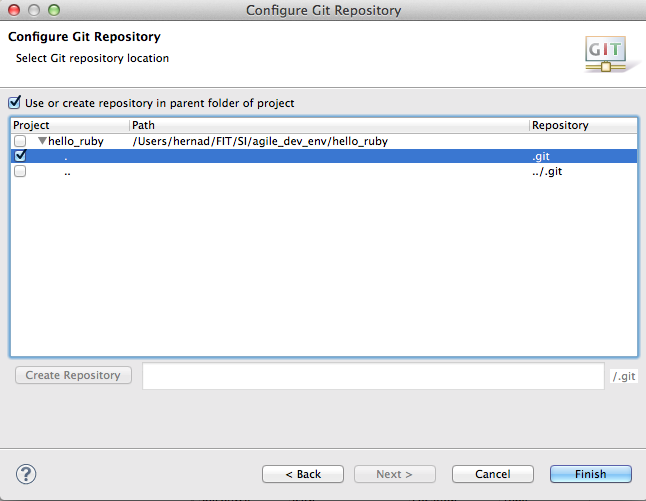
\includegraphics[width=10cm]{img/eclipse_git_01.png}
\caption{Eclipse IDE git - setup postojećeg repozitorija u IDE-u}
\end{figure}

Nakon toga su nam dostupne SCM operacije nad repozitorijom:
\begin{figure}[H]
\centering
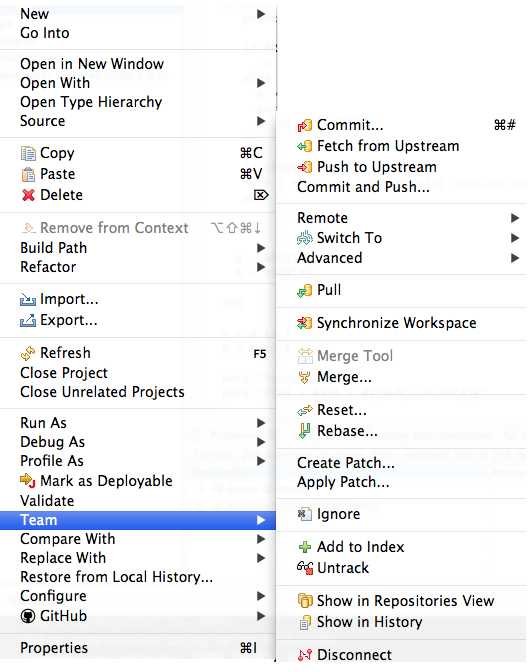
\includegraphics[width=10cm]{img/eclipse_git_02.png}
\caption{Eclipse IDE GIT - Project team support}
\end{figure}

Nakon izvršenih promjena unutar IDE-a, pokrećemo commit unutar IDE-a:
\begin{figure}[H]
\centering
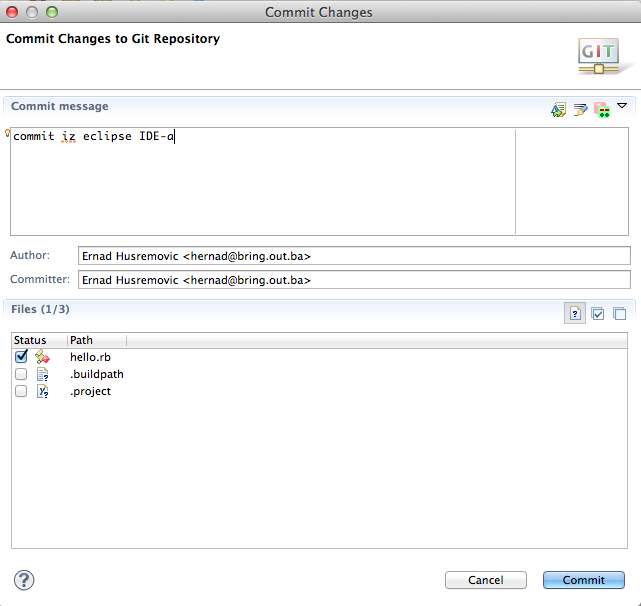
\includegraphics[width=12cm]{img/eclipse_git_03.png}
\caption{Eclipse IDE commit dijalog}
\end{figure}

Push na remote repozitorij:

\begin{figure}[H]
\centering
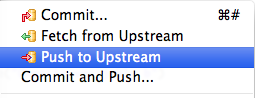
\includegraphics[width=5cm]{img/eclipse_git_04.png}
\caption{Eclipse push dijalog}
\end{figure}

\begin{figure}[H]
\centering
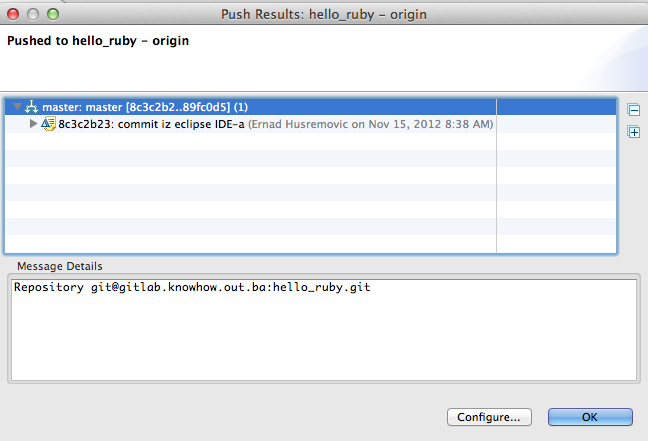
\includegraphics[width=10cm]{img/eclipse_git_05.png}
\caption{Eclipse IDE, informacija o izvršenoj push operaciji}
\end{figure}


\begin{figure}[H]
\centering
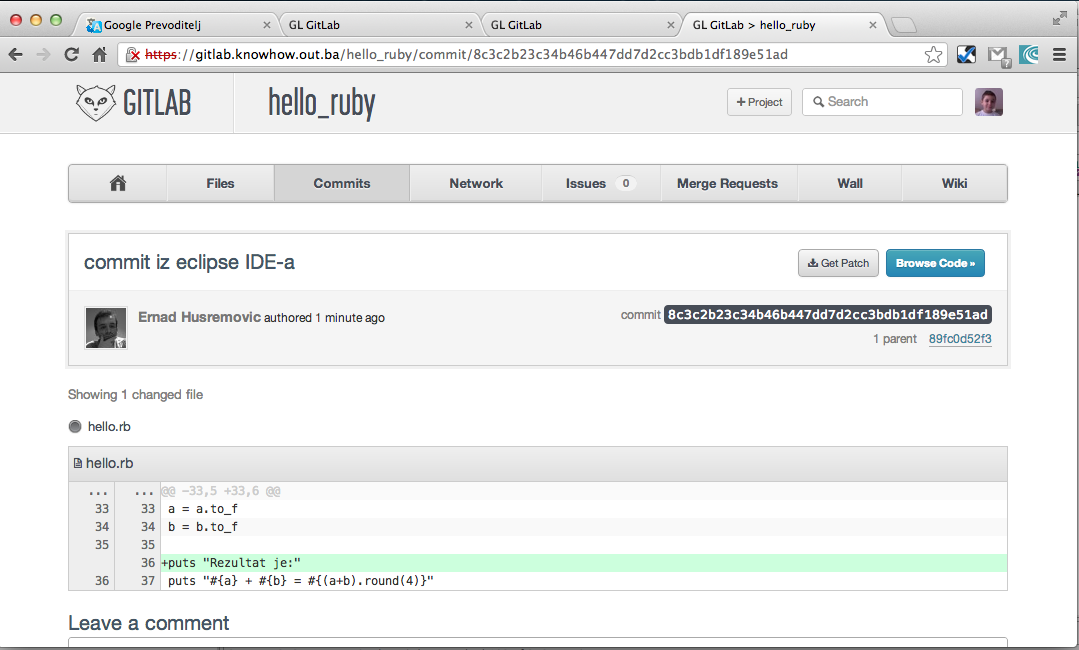
\includegraphics[width=15cm]{img/eclipse_git_06.png}
\caption{Naša promjena nalazi se na gitlab serveru}
\end{figure}

\section{''Collective code ownership''}

\begin{quotation}
  \emph{We are all responsible for high-quality code.}
\end{quotation}

''Collective code ownership''\citep[str. ]{agileart} je agilni princip po kome svako odgovoran za visoki kvalitet koda.
Ako se tokom čitanja uputstva uoče nedostaci, ako je programski kod nepregledan, pristupa se popravci.
Pri tome se ne gleda ko je originalni pisac uputstva ili koda. Kod je u vlasništvu tima.

Ernad je nakon Bakirovih intervencija na uputstvu uočio da postoji još par stavki koje bi trebalo ispraviti.

Za ovu intervenciju nema nikakvog razloga praviti novi branch - ispravke će se vršiti direktno u ''master''-u.

Ernad vrši update master-a na svom desktopu:

hernad@hello\ruby\$ \texttt{git checkout master}
\begin{lstlisting}
Switched to branch 'master'
Your branch is behind 'origin/master' by 6 commits, and can be fast-forwarded.
\end{lstlisting}

Ernad preuzima (pull-uje) Bakir-ove promjene sa servera:

hernad@hello\ruby\$ \texttt{git pull}
\begin{lstlisting}
Updating feab5f1..1ed5b06
Fast-forward
 README.md |   34 +++++++++++++++++++++++++++++++++-
 hello.rb  |   38 ++++++++++++++++++++++++++++++++------
 2 files changed, 65 insertions(+), 7 deletions(-)
\end{lstlisting}

Vriš ispravku uputstva u svom editoru:

hernad@hello\ruby\$ \texttt{vi README.md}
\begin{lstlisting}
Commit-uje promjene:
\end{lstlisting}

hernad@hello\ruby\$ \texttt{git commit -a}
\begin{lstlisting}
[master 74fb346] uputstvo update
 1 file changed, 1 insertion(+), 1 deletion(-)
\end{lstlisting}

Označava novu verziju 0.3.2:

hernad@hello\ruby\$ \texttt{git tag 0.3.2}

hernad@hello\ruby\$ \texttt{git push origin master --tags}
\begin{lstlisting}
Counting objects: 5, done.
Delta compression using up to 8 threads.
Compressing objects: 100% (3/3), done.
Writing objects: 100% (3/3), 333 bytes, done.
Total 3 (delta 1), reused 0 (delta 0)
To git@gitlab.knowhow.out.ba:hello_ruby.git
   1ed5b06..74fb346  master -> master
 * [new tag]         0.3.2 -> 0.3.2
\end{lstlisting}

Treba uočiti da je ovaj proces brz i jednostavan. Ne traži nikakve posebne dogovore između developera.
Jednostavno, svako ko uoči potrebu da napravi sitnu korekciju - to i čini.

\chapter{Zaključak}

Git nam omogućava da se jedan od ključnih prinicipa agilnog sofware dvelopmenta, ''Collective code ownership'', realizira u praksi.

Git omogućava developeru da sve svoje ideje sa minimalnim ''overhead''-om pohrani u centralni repozitorij (branching).

Web servisi kao što su Github i Gitlab omogućavaju jednostavnu i efikasnu komunikaciju tima. Centralna tačka komunikacije je izvorni kod\footnote{Ovdje se misli na izvorni kod u širem smislu. Misli se na sve digitalne artifakte projekta. Dokumentacija je sastavni dio izvornog koda}.
Kako je izvorni kod projekta je glavni proizvod programskog tima, to je i prirodno mjesto komunikacije.

Pored mogućnosti da se direktno ispravlja programski koda, svaki član tima ima mogućnost komentara pojedinih ''commit''-a.

Ta opcija omogućava iskusnijim članovima tima (senior developer, product manager, agile couch) da junior programerima brzo i jednostavno daju upute za korekcije i nadogradnju njihovog koda.


%\begin{center}
%\emph{\large{Freedom to create, distribute, and use open source software (OSS).}}
%\end{center}


% -------------------------------------------------
\bibliography{literatura}
\bibliographystyle{fit}

% -------------------------------------------------
\appendix

\chapter{Riječnik pojmova}

\begin{itemize}
    \item \texttt{tag} - tag je oznaka unutar git repozitorija koja najčešće pokazuje na određenu verziju (release) ili podverziju - iteraciju (iteration)

    \item \texttt{branch} - branch označava poseban ogranak projekat u odnosu na glavni tok razvoja. Primjera radi, ako želimo uvesti neke eksperimentalne funkcije, otvaramo poseban "experimental" branch unutar koga implementiramo naše eksperimentalne funkcije. Te promjene se ne vide na glavnom - ''master'' branch-u.
    \item \texttt{merge request} - Proces merdžiranja (eng. merge - spojiti) je proces u kome se vrši spajanje promjena iz različiti branch-ova ili različitih repozotorija. Vezano za primjer branch-a (vidi: branch), ako su se promjene u ''experimental'' branch-u pokazale dobrim, ''merge'' operacijom ih prebacujemo - integriramo u ''master'' branch. Nakon uspješnog merdžiranja ''experimental'' branch možemo obrisati.
   \item \texttt{repository} - baza u promjena. Lokalni repozitorij se nalazi u .git repozitoriju našeg projekta na lokalnom disku. 'Remote' repozitorij se uobičajeno nalazi na udaljenom serveru kome pristupamo putsem ssh ili http protokola.
\end{itemize}

\chapter{Napomene}

Materijal je prepun anglizama, što odstupa od uobičajenih akademskih standarda pisanja. Međutim, s obzirom na ciljni auditorij, mišljenja smo da bi pokušaj prevođenja na maternji jezik izazvao više konfuzije nego što bi pomogao u razumjevanju sadržaja.

Uzmimo za primjer \href{http://translate.google.com/#en/hr/commit}{\color{blue}{''commit''}} operaciju.
Uzevši u obzir kontekst, ''commit'' operacijom se promjene šalju - predaju u lokalni repozitorij.
Stoga bi prevod najadekvatnije bilo koristiti riječ ''predaj'' na bosanskom jeziku.
Koliko bi prevoda ovih termina bio neprimjeren, zorno pokazuje pokušaj prevoda opcija na sljedećem ekranu:

\begin{figure}[H]
\centering
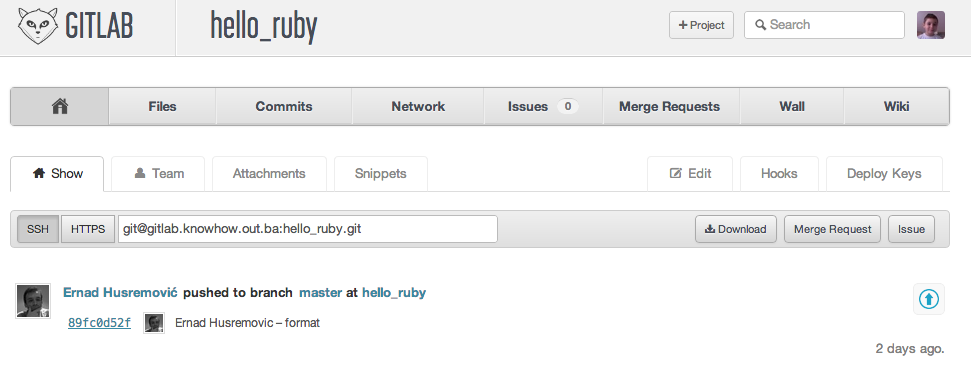
\includegraphics[width=16cm]{img/cik_prevedi.png}
\caption{Prevod na bosanski - nemoguća misija}
\end{figure}

Stoga se termini ''hardware'', ''software'', ''commit'', ''push'', ''merge'', ''branch'' u materijalu koriste isključivo u izvornoj formi.

\chapter{Software toolset}
\begin{enumerate}
  \item Mac OS X 10.8.2
  \item mvim, vim tekst editor ver 7.3
  \item MacTex (TeX Live 2012)
\end{enumerate}

\chapter{Software repozitoriji}

\begin{itemize}
  \item Agilni developerski environment  \url{https://github.com/hernad/agile\_dev\_env}

\end{itemize}

\end{document}
